\title{Note on estimating the error of the extracted time resolution}
\date{August 05, 2015}

\documentclass[12pt]{article}

\usepackage{hyperref}
\usepackage{cite}

\usepackage{graphicx}
\usepackage{epsfig}
\usepackage{epstopdf}

\usepackage[pdf]{pstricks}

\usepackage{mathtools}
\newcommand{\defeq}{\vcentcolon=}

\usepackage{float}
\restylefloat{table}

%! To create a place-holder figure
\newcommand{\dummyfig}[1]{
  \centering
  \fbox{
    \begin{minipage}[c][0.33\textheight][c]{0.5\textwidth}
      \centering{#1}
    \end{minipage}
  }
}

\begin{document}
\maketitle

% \begin{abstract}
% This is the paper's abstract \ldots
% \end{abstract}

 
\section{Introduction}

Estimating the error of the extracted time resolution of the system requires a thorough analysis of the statistical and non-statistical uncertainties. Given the scale of the project and therefore, constraints on the time, it was not possible to perform such an analysis for each of the sets of counters. In this section we present a detailed analysis of the error estimate using a set of reference counters -- 6x210cm bars(half slow, half fast) and 1st article PMTs -- and describe the method we used to extrapolate the obtained result to counters of all lengths.

\subsection{Time resolution measurement and its error along the length of a bar}
For each bar length, even after 2 days of data taking, the statistics in the T histogram (\textit{refer to formula in doc.}) are low and therefore, the statistical methods that can be used to fit and obtain the standard deviation of these histograms, which is the time resolution, has to be studied, since each method, in the low statistic limit, has its own limitation in estimating the true standard deviation and its error. 

Figure 1. shows the statistics accumulated (N) for the shortest and longest counters versus points along the bar. Figures 2. and 3. show a comparison of the various fitting methods available in ROOT for extracting $\mu$ and $\sigma$ from simulated Gaussian histograms ($\mu_{T}$ and $\sigma_{T}$) for N values between 100 and 600, reflecting the low and high end of the statistics versus bar length (as can be seen in Figure 1.). The range of simulated $\sigma_{T}$, similarly, covers the low and high end of the typical standard deviation values expected from the FTOF12 system, corresponding to the shortest and longest bars, respectively (\textit{confirm this!}).

\begin{figure*}[ht]
	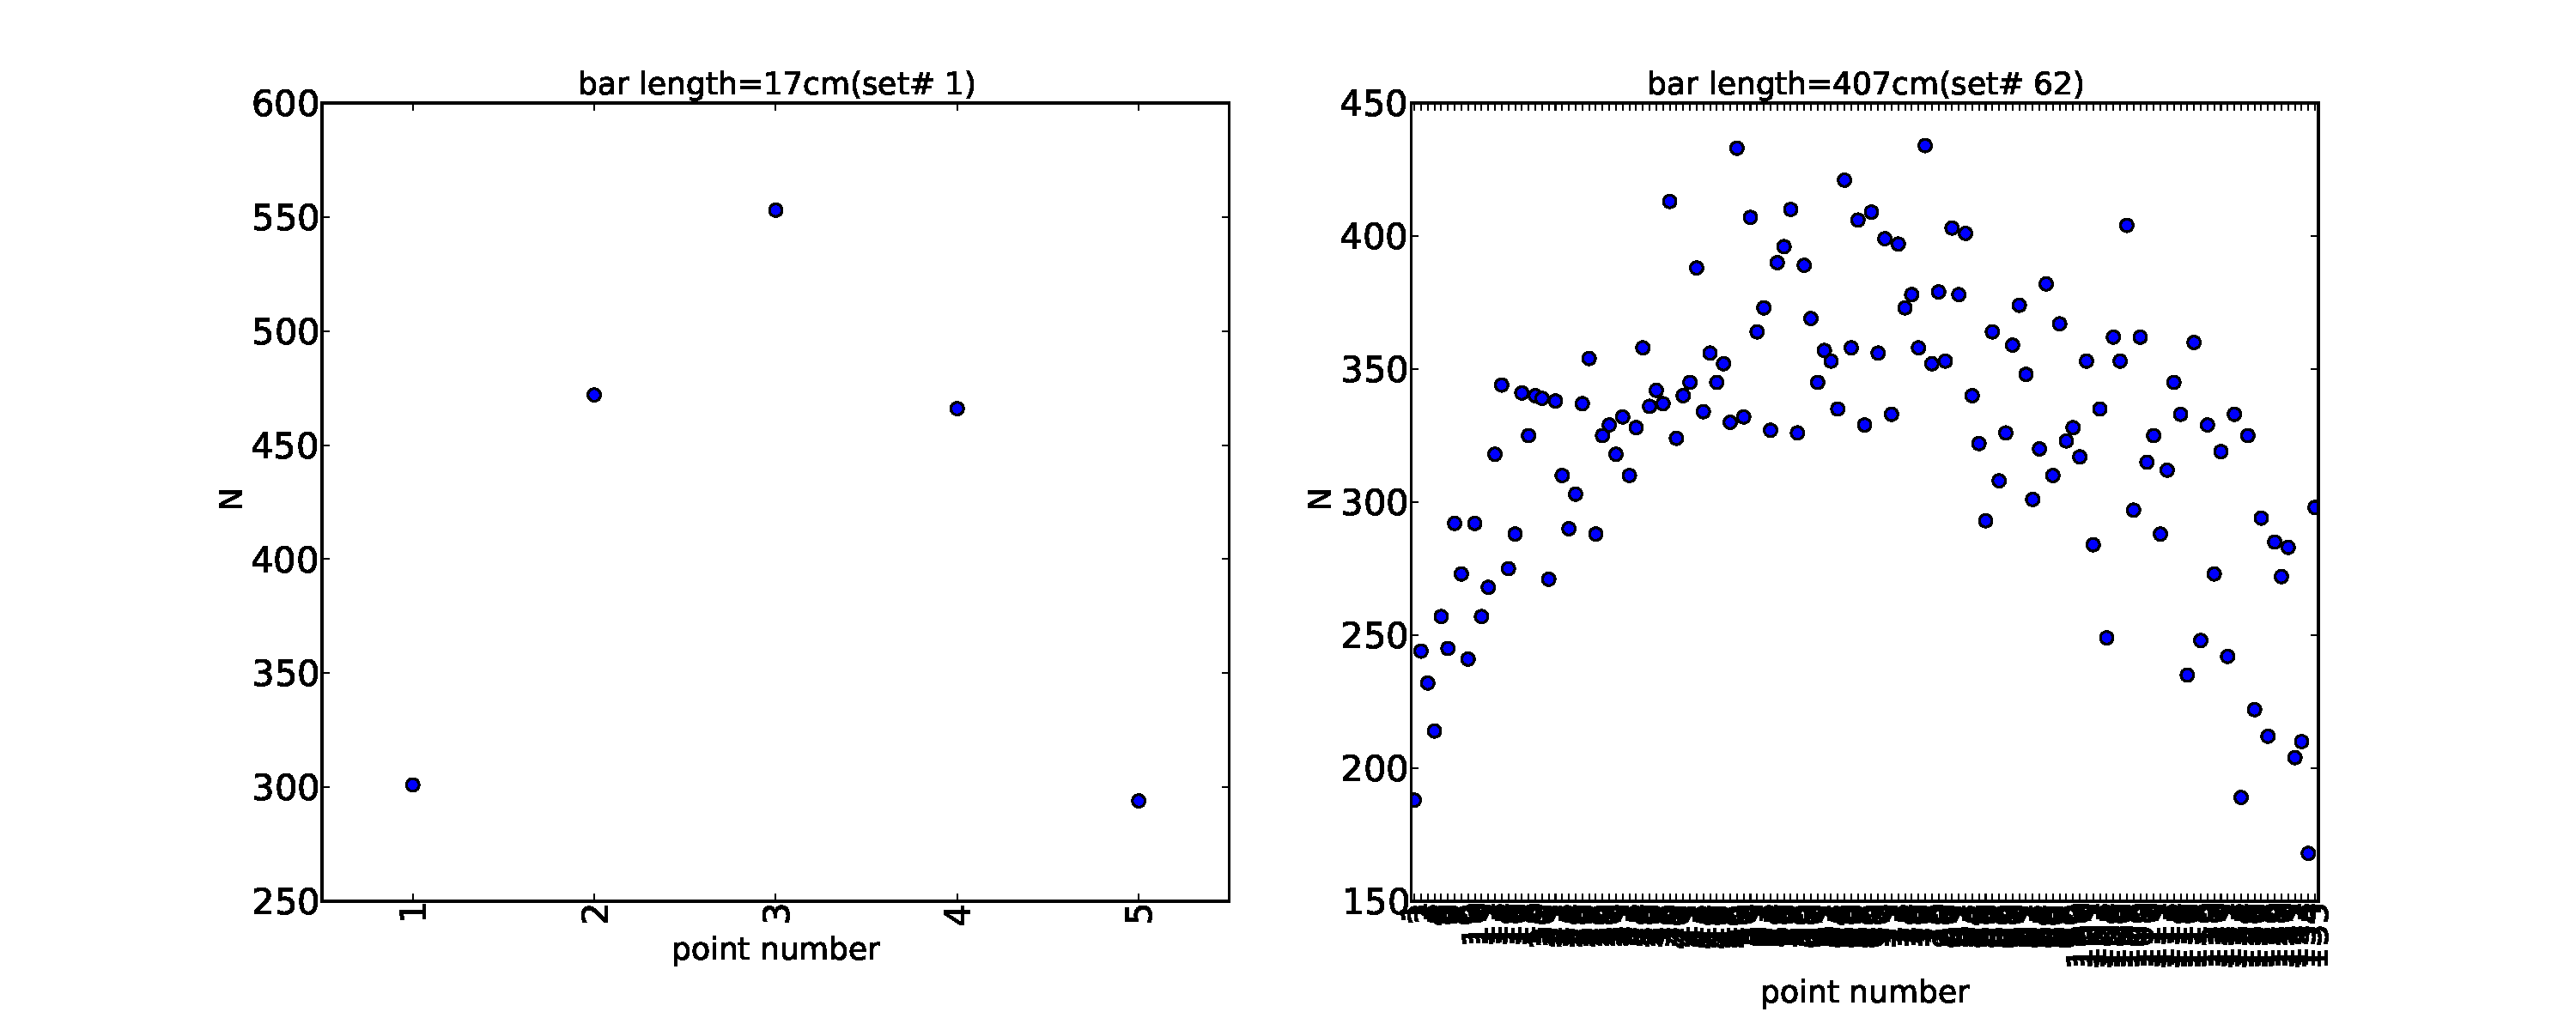
\includegraphics[height=2in,width=5in]{bar_stats_write-up_N-vs-p.pdf}
	\caption{N vs. P for the shortest and longest counters}
	\label{fig1}
\end{figure*}

Figure 2. is a comparison of the Chi-square(CSQ) method with Maximum Likelihood(MLE). It is observed that the CSQ fit results for $\sigma_{T}$ are neither accurate nor stable in the low N region and this gets worse as the ratio of $\frac{\sigma_{T}}{N}$ increases. It turns out that for most of the N region of interest for the FTOF12 system, the $\sigma_{T}$ obtained by CSQ is mostly underestimated by $\approx$ 2\%, however, if N gets low enough, or alternatively $\frac{\sigma_{T}}{N}$ get high enough, the instability of the results may cause an overestimation of the $\sigma_{T}$ by amounts that vary with $\frac{\sigma_{T}}{N}$, worsening as this ratio increases. It is also important to note, especially for the case of an automated analysis program, that the instability of the CSQ in the low N region also leads to cases where the method fails in its execution. The $\sigma_{T}$ obtained by the MLE fit, on the other hand, is stable and accurate up to $\approx$ 1\%

The $\mu_{T}$ extracted from both methods are in agreement within statistical uncertainties, however, it is not used in extracting the time resolution.

While this study clearly establishes the superiority of the MLE method in the low N limit, it is not suited for the extraction of the time resolution for a large scale system. The measured data contains data points that are ``outliers'' to the T-distribution and to which the MLE method is highly sensitive, making it estimate a higher standard deviation (\textit{Fig 4. will demonstrate this once its updated with the MLE analysis}). The unpredictabe nature of the ``outliers'' and the large dynamic range over which the T-distributions can appear, which is additionally affected by the test setup, make it impossible, at least a priori, to specify an appropriate fitting range in an automated analysis program.

The other remaining option is to use a modified version of the CSQ fit in ROOT (CSQ-WW) where the error bars in the histogram bins are ignored(\textit{Confirm this at the code level in ROOT and if indeed the documentation in ROOT for WW, ``set weights in all bins to 1;ignore error bars'' means this}). CSQ-WW is observed to effectively perform like MLE, but the error on the $\mu_{T}$ and $\sigma_{T}$ estimate, in comparison, is lower. Additionally, it is biased in its estimation of $\sigma_{T}$ for very low N, $\approx$ 2\% understimation of $\sigma_{T}$ (\textit{May be I have conservatively simulated too low an N value and I should make it more realistic -- N$>$150 as per Fig. 1 -- and then this statement will no longer be needed}). Fig. 3 shows the extracted parameters from the CSQ-WW option compared with CSQ. (\textit{Should generate a direct comparison with MLE})

\begin{figure*}[ht]
	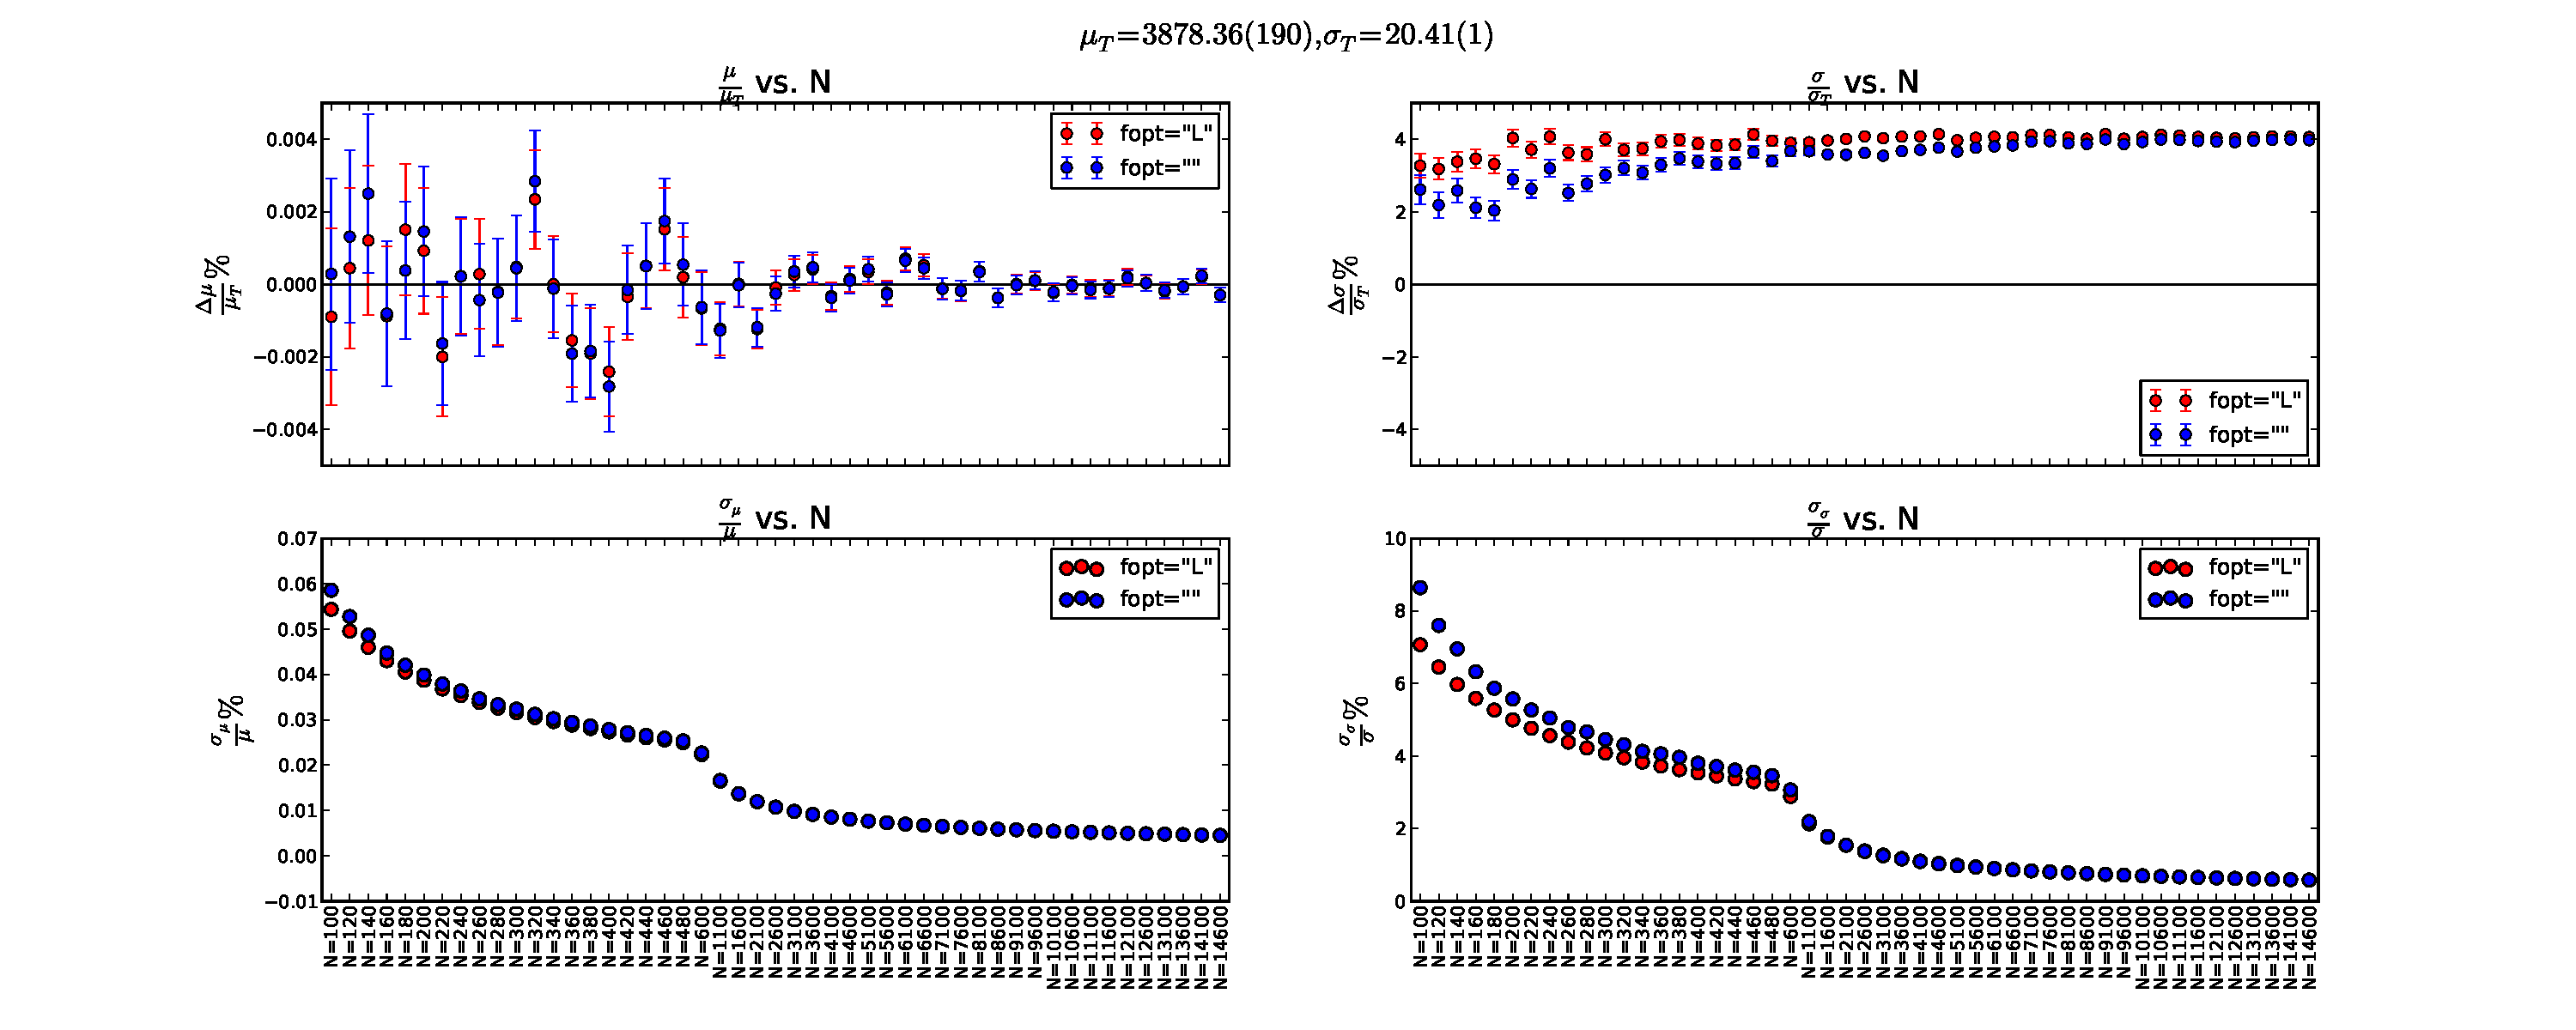
\includegraphics[height=2.5in,width=5.5in]{fit-comp_MU-190_SG-1_fit-opt-L_binw-1.pdf}
	%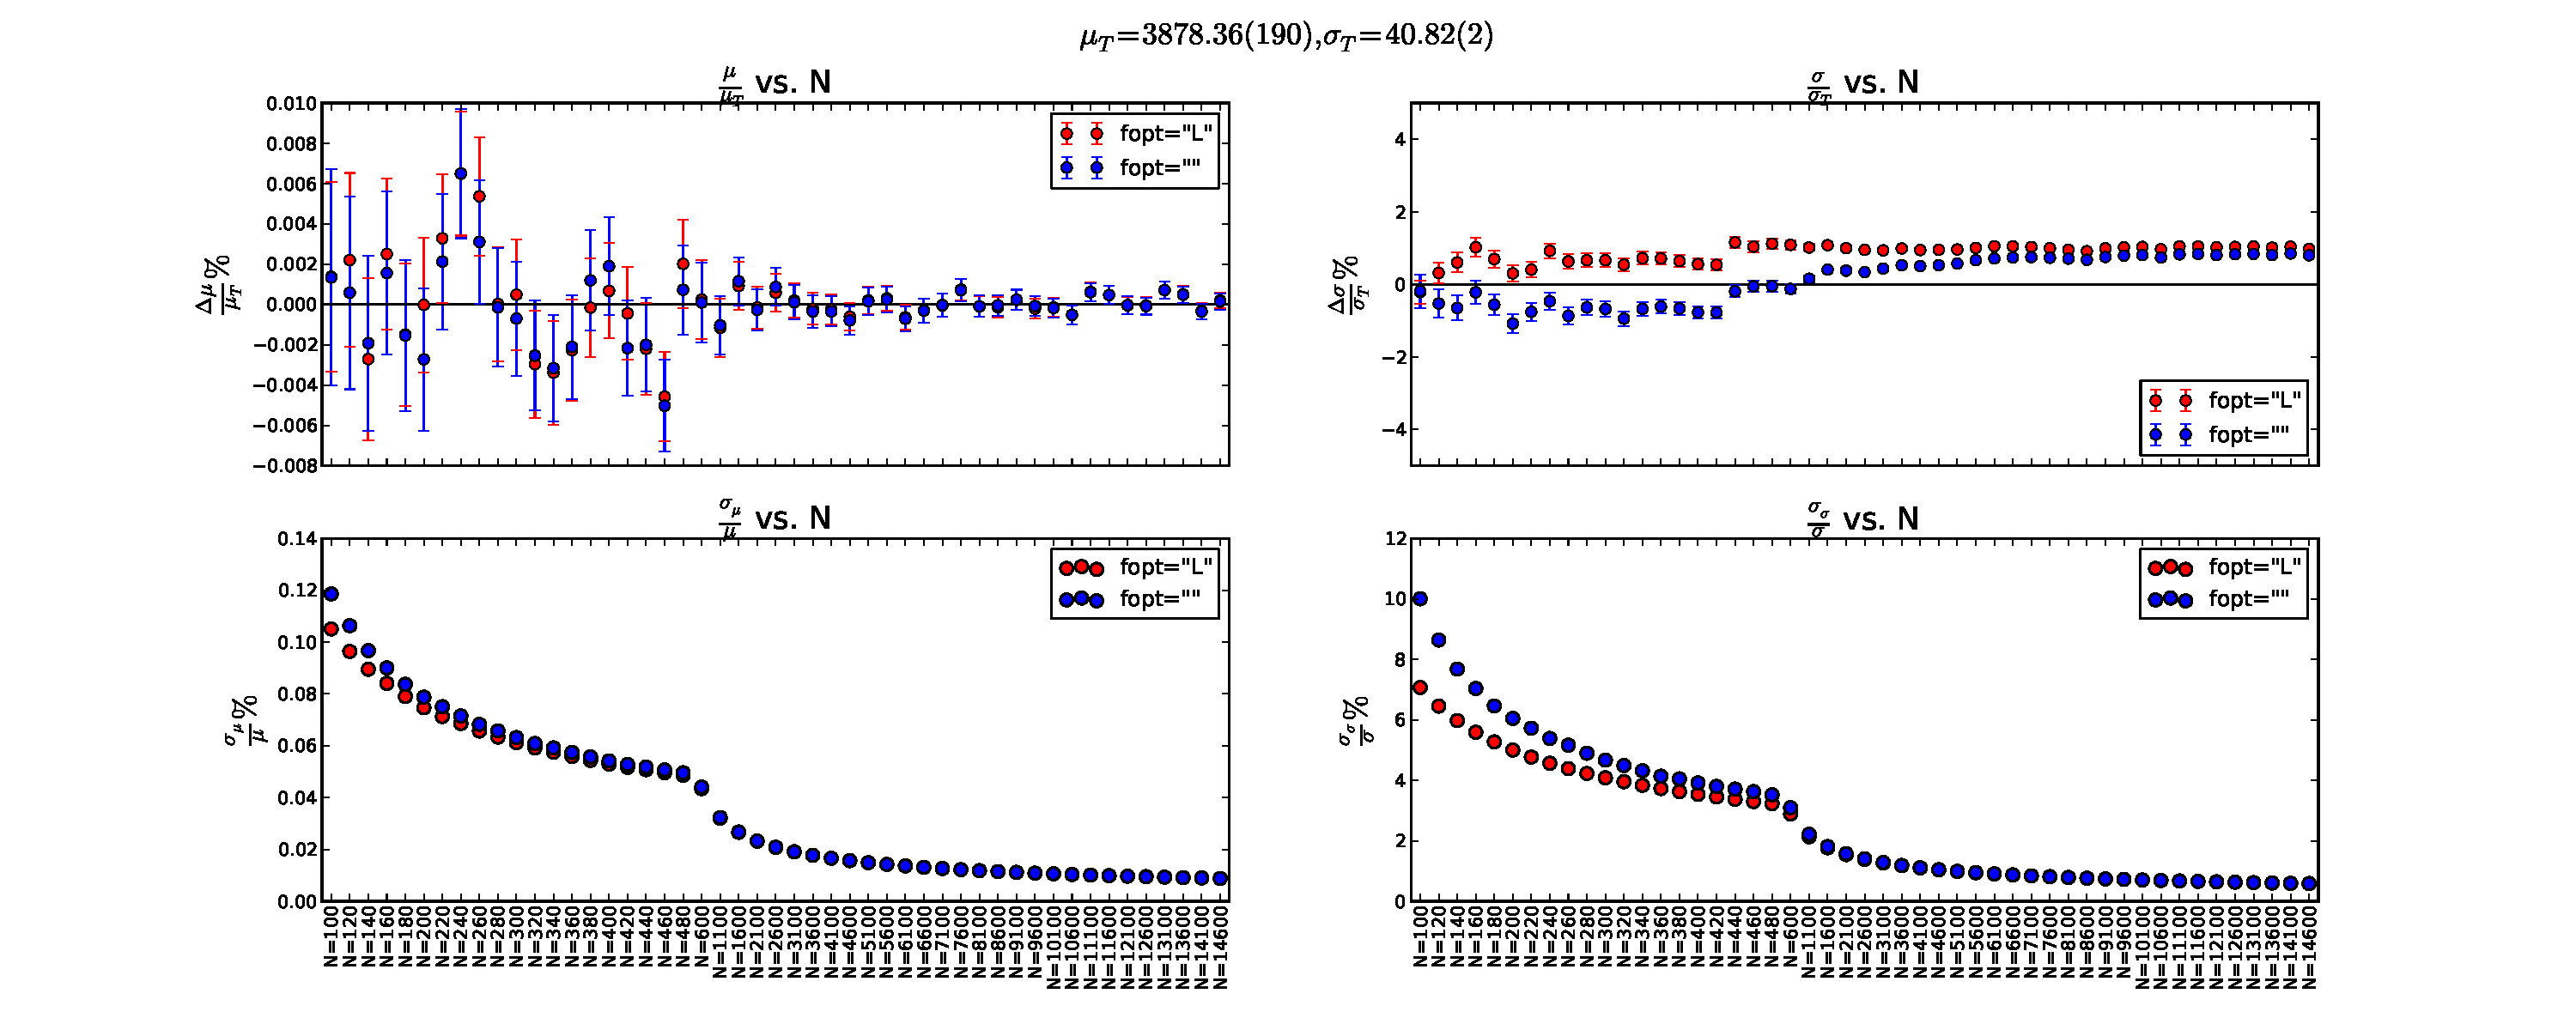
\includegraphics[height=2.5in,width=5.5in]{fit-comp_MU-190_SG-2_fit-opt-L_binw-1.pdf}
	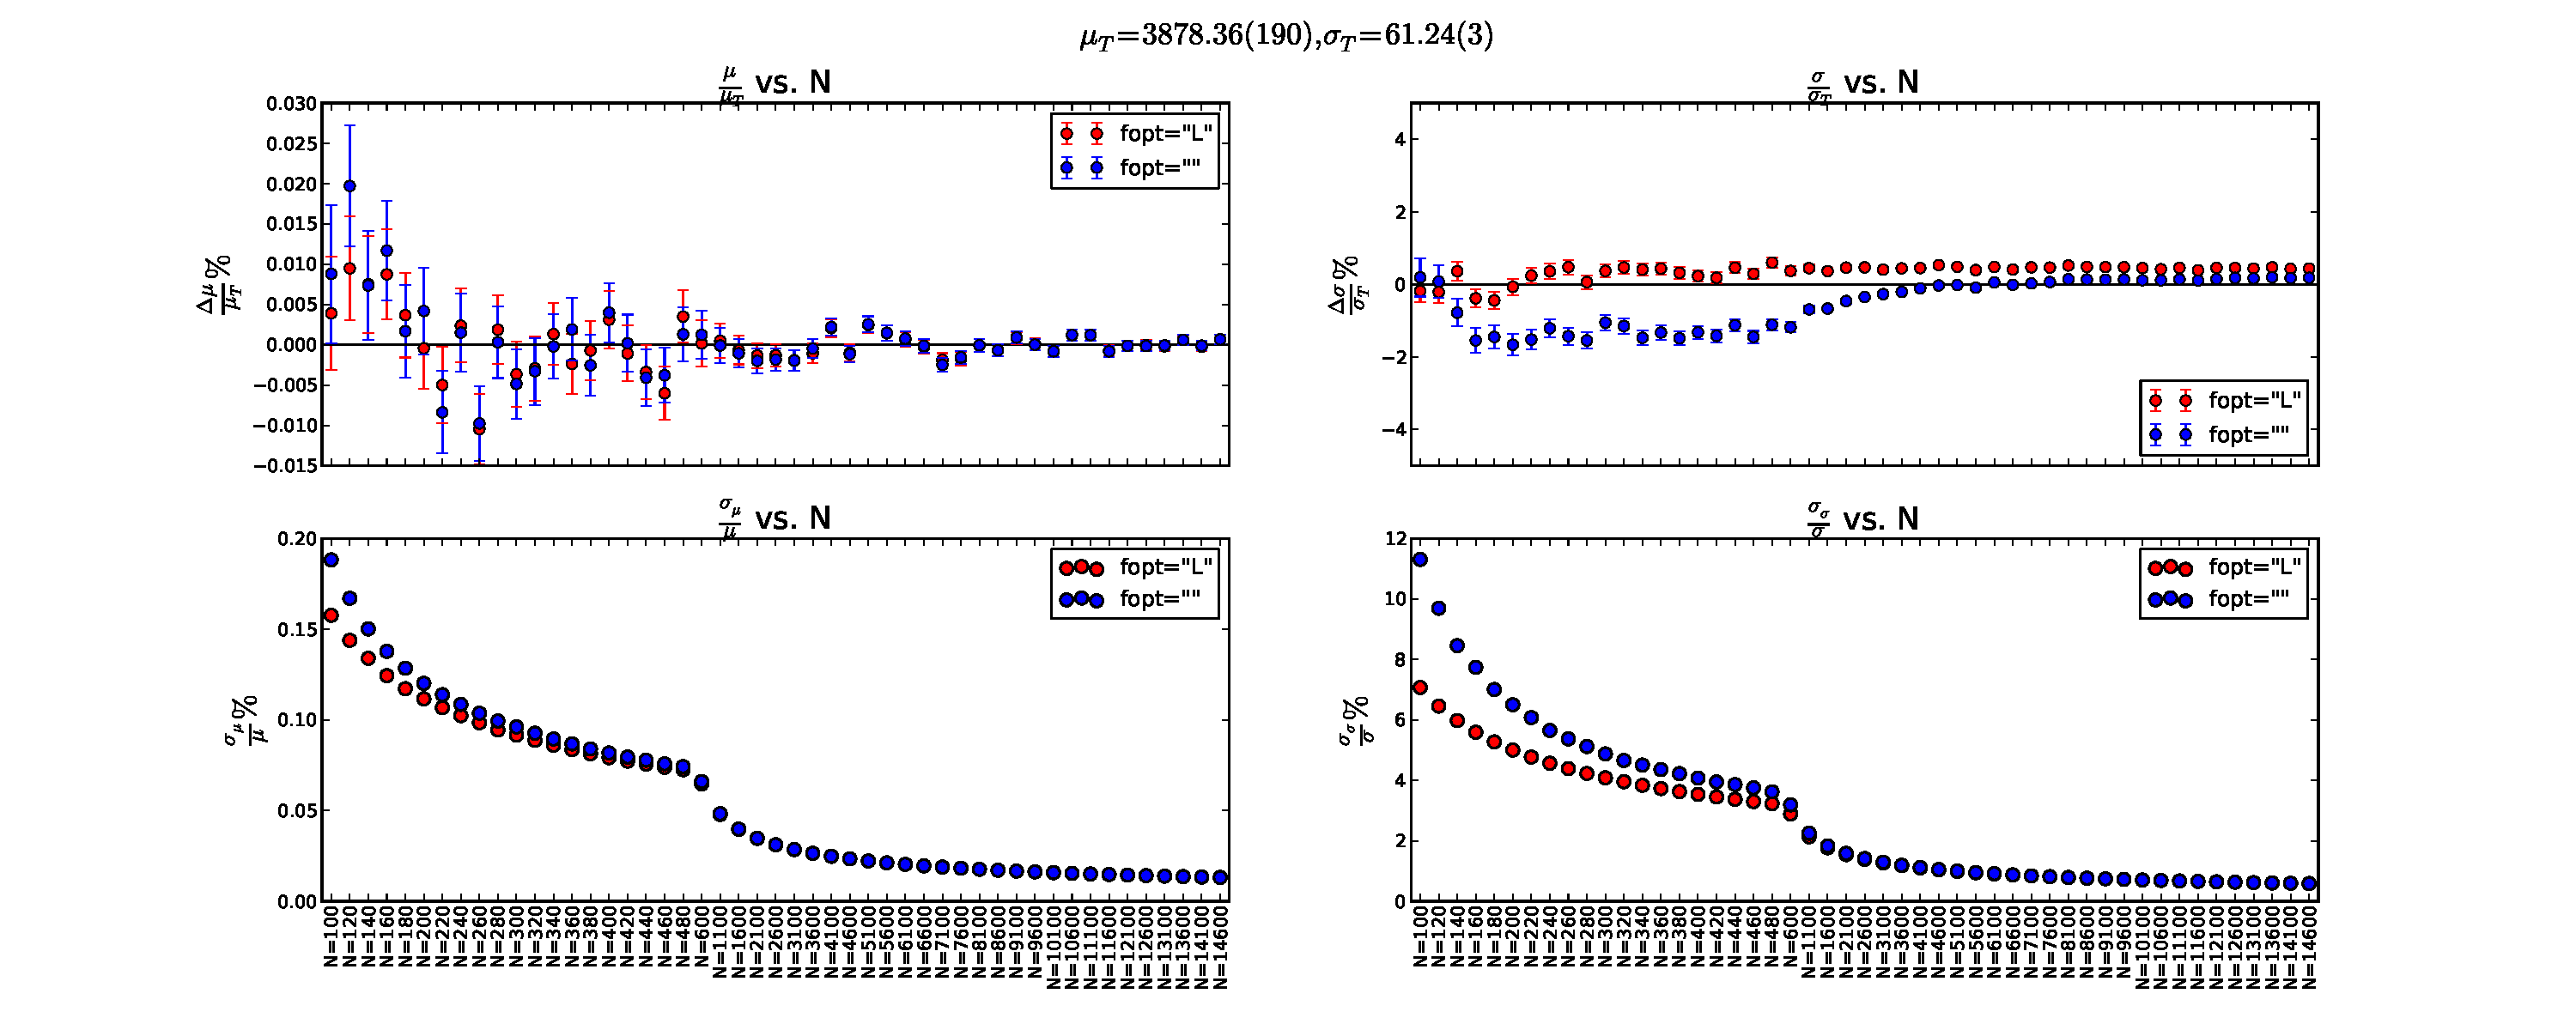
\includegraphics[height=2.5in,width=5.5in]{fit-comp_MU-190_SG-3_fit-opt-L_binw-1.pdf}
	%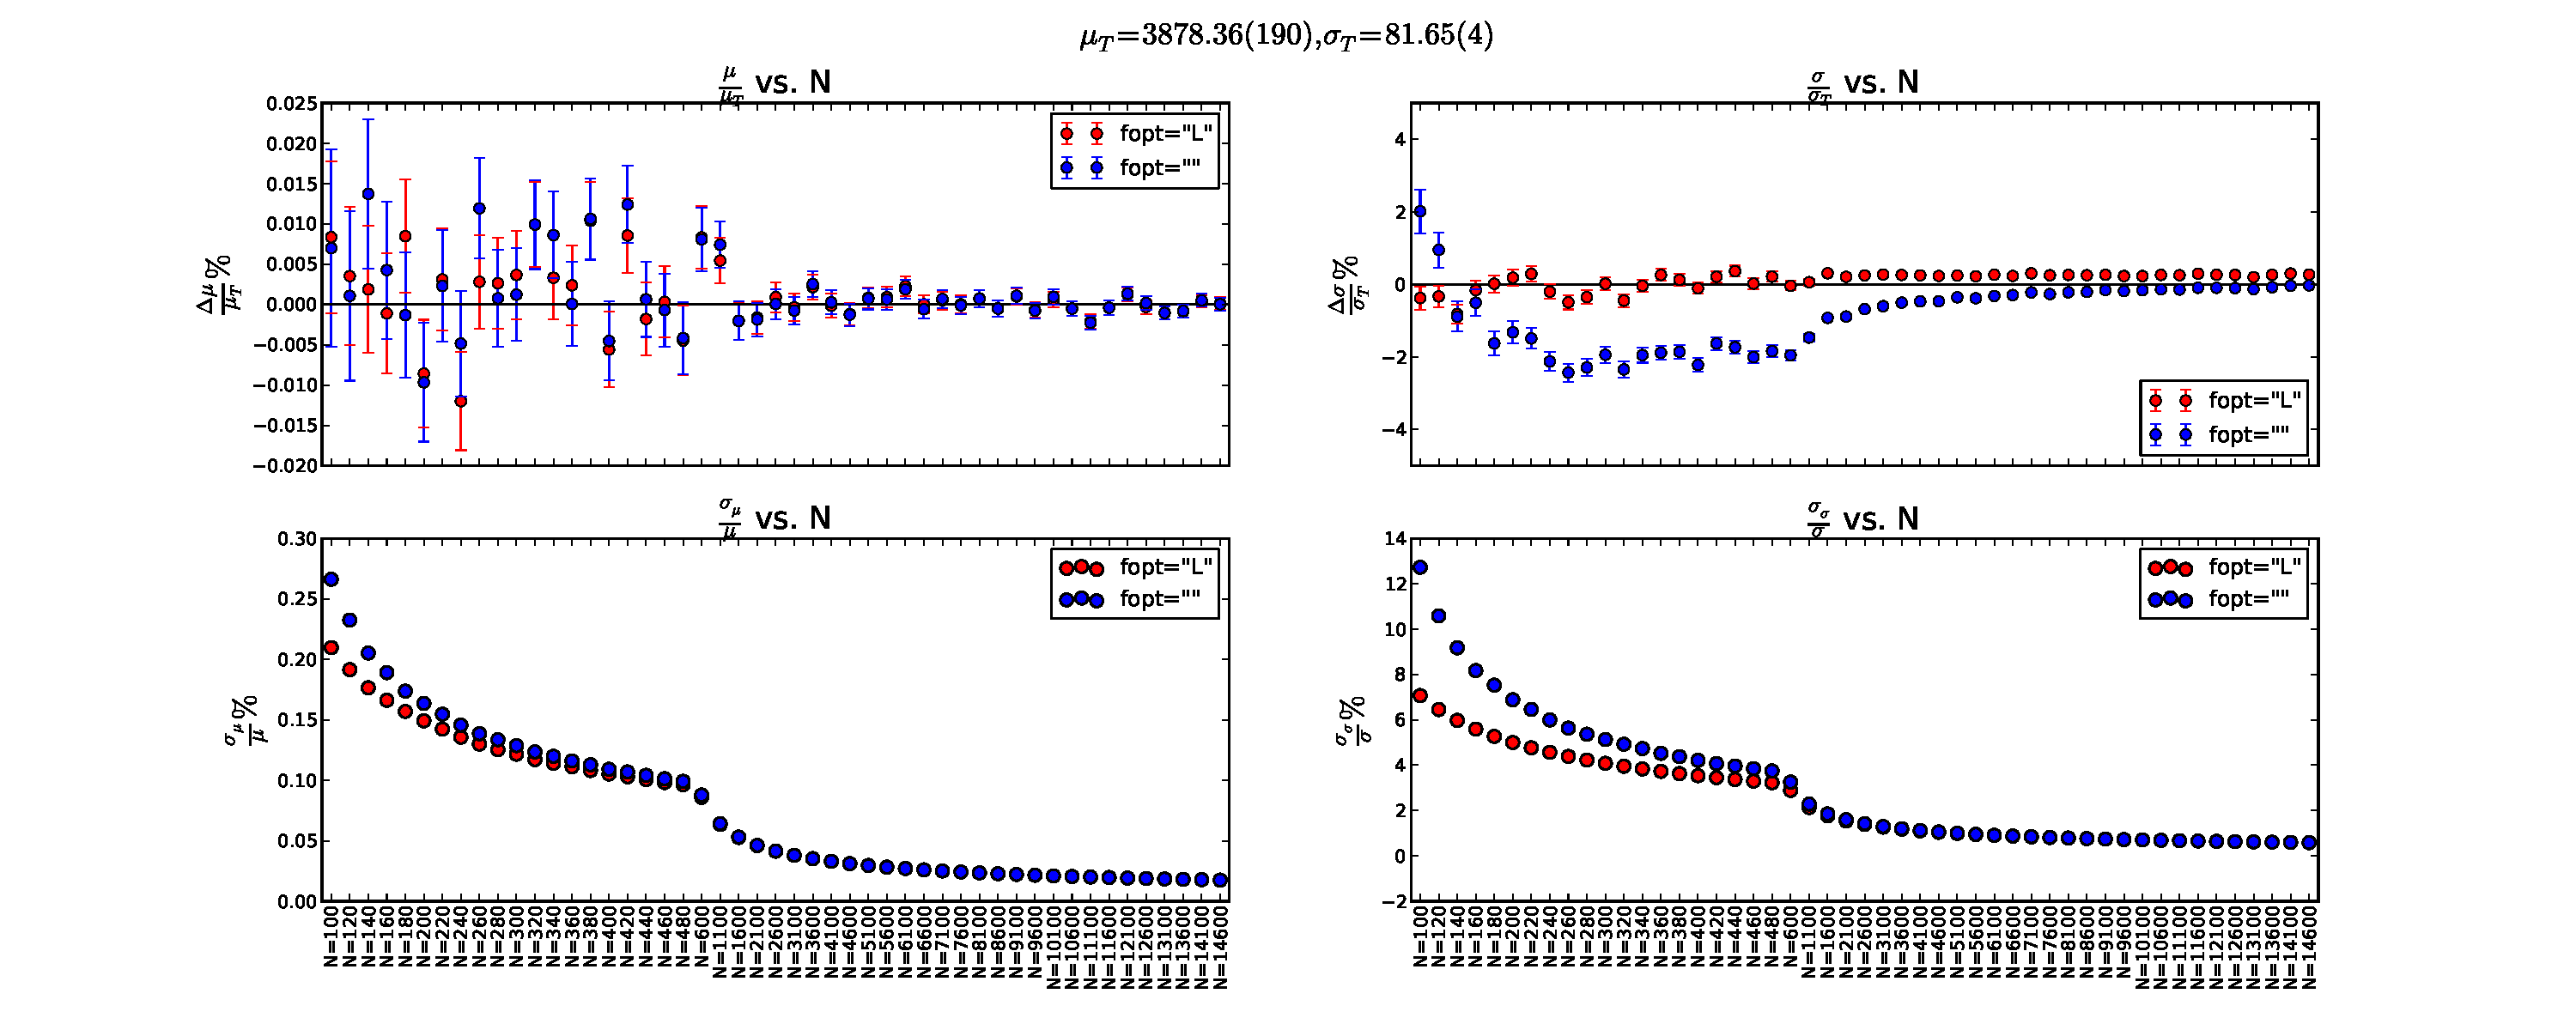
\includegraphics[height=2.5in,width=5.5in]{fit-comp_MU-190_SG-4_fit-opt-L_binw-1.pdf}
	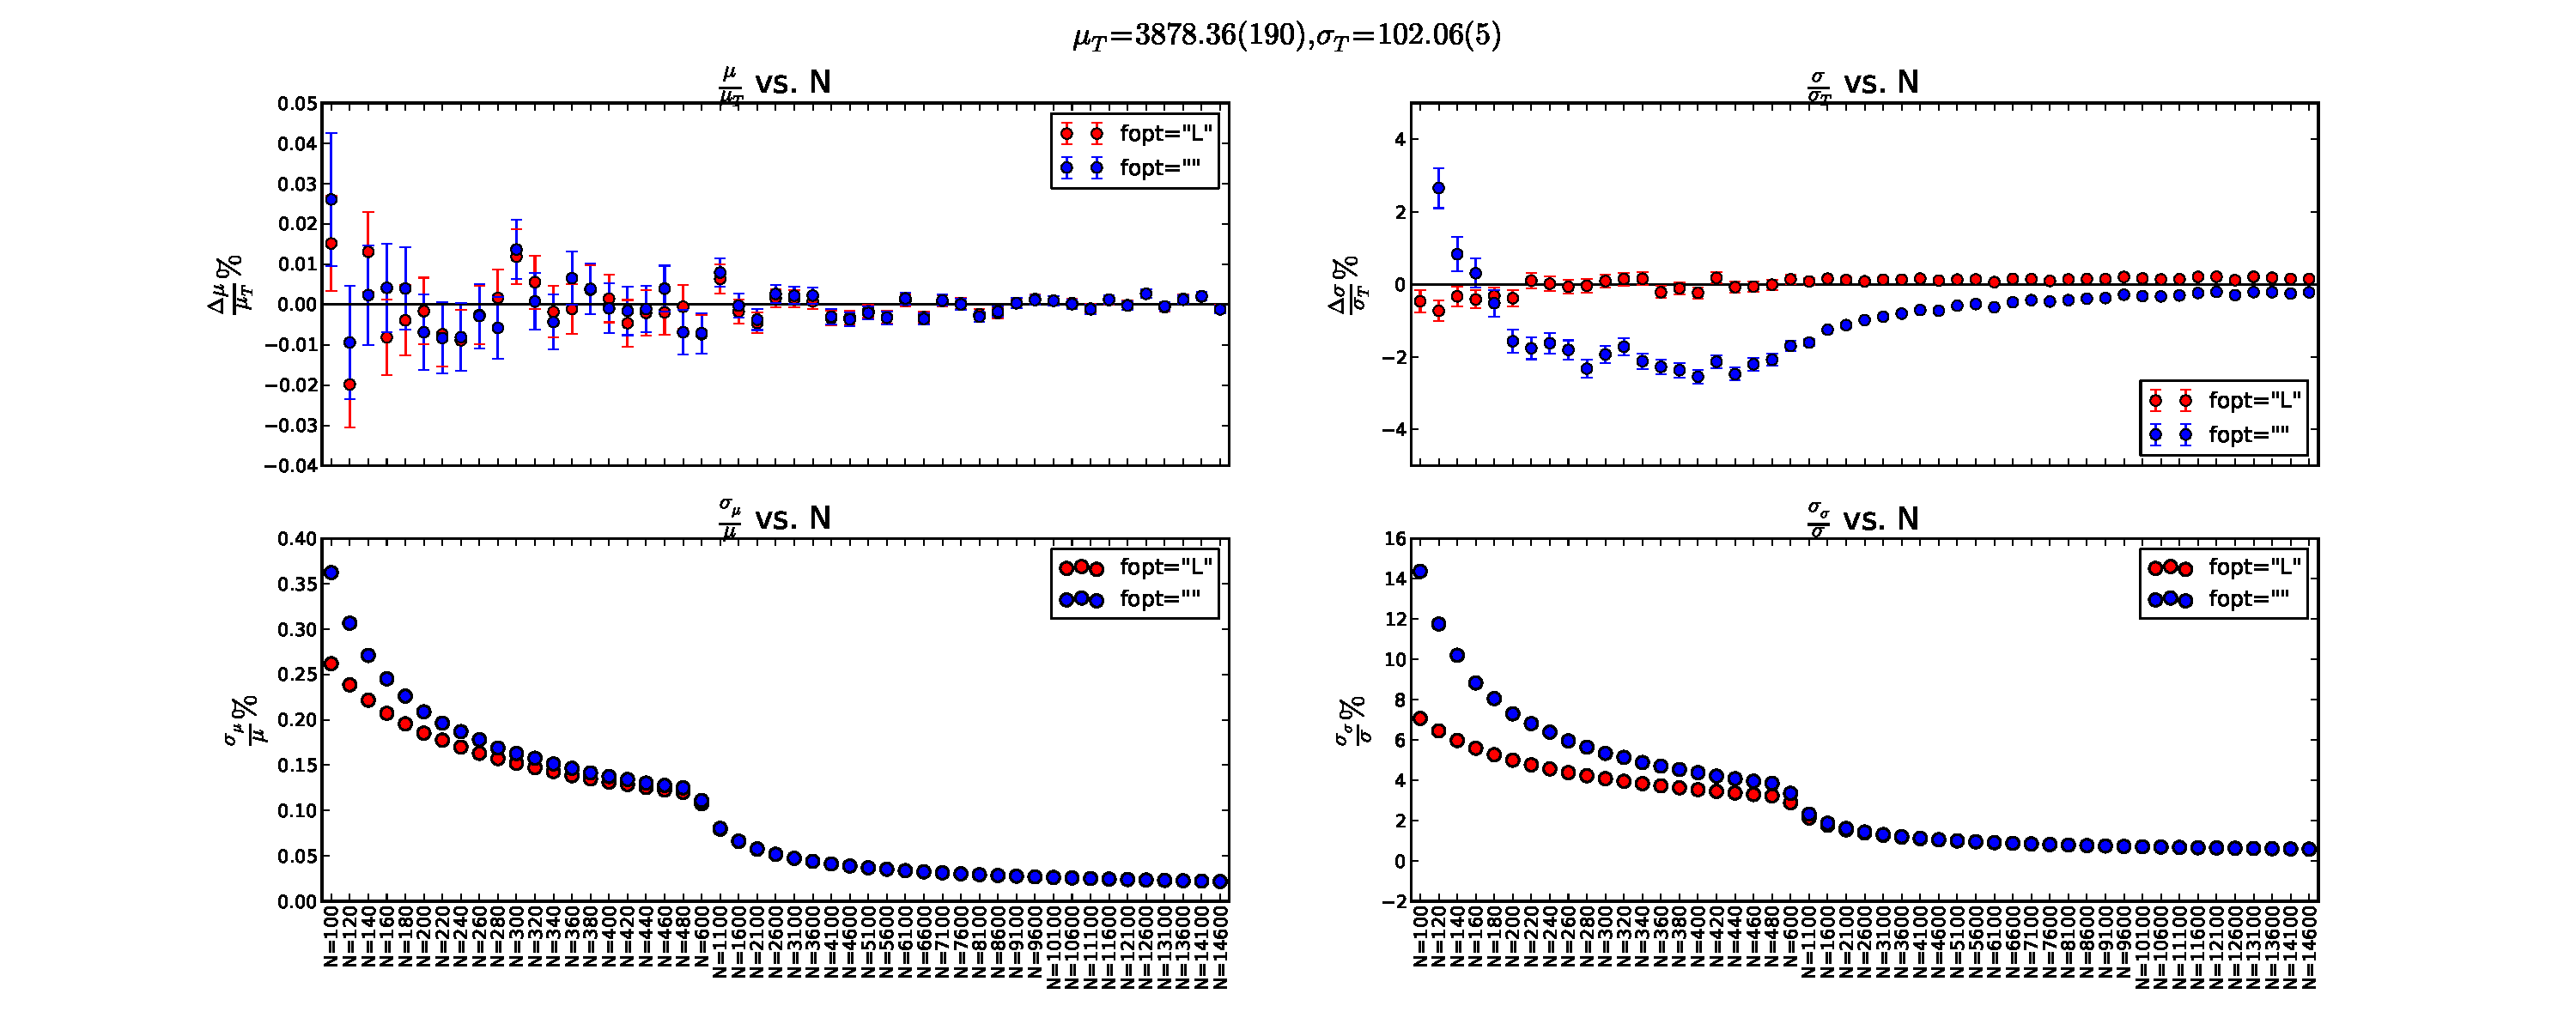
\includegraphics[height=2.5in,width=5.5in]{fit-comp_MU-190_SG-5_fit-opt-L_binw-1.pdf}
	\caption{Extracted parameters (MLE and CSQ) as a function of N and $\sigma_{T}$}
	\label{fig2}
\end{figure*}

\clearpage

\begin{figure*}[ht]
	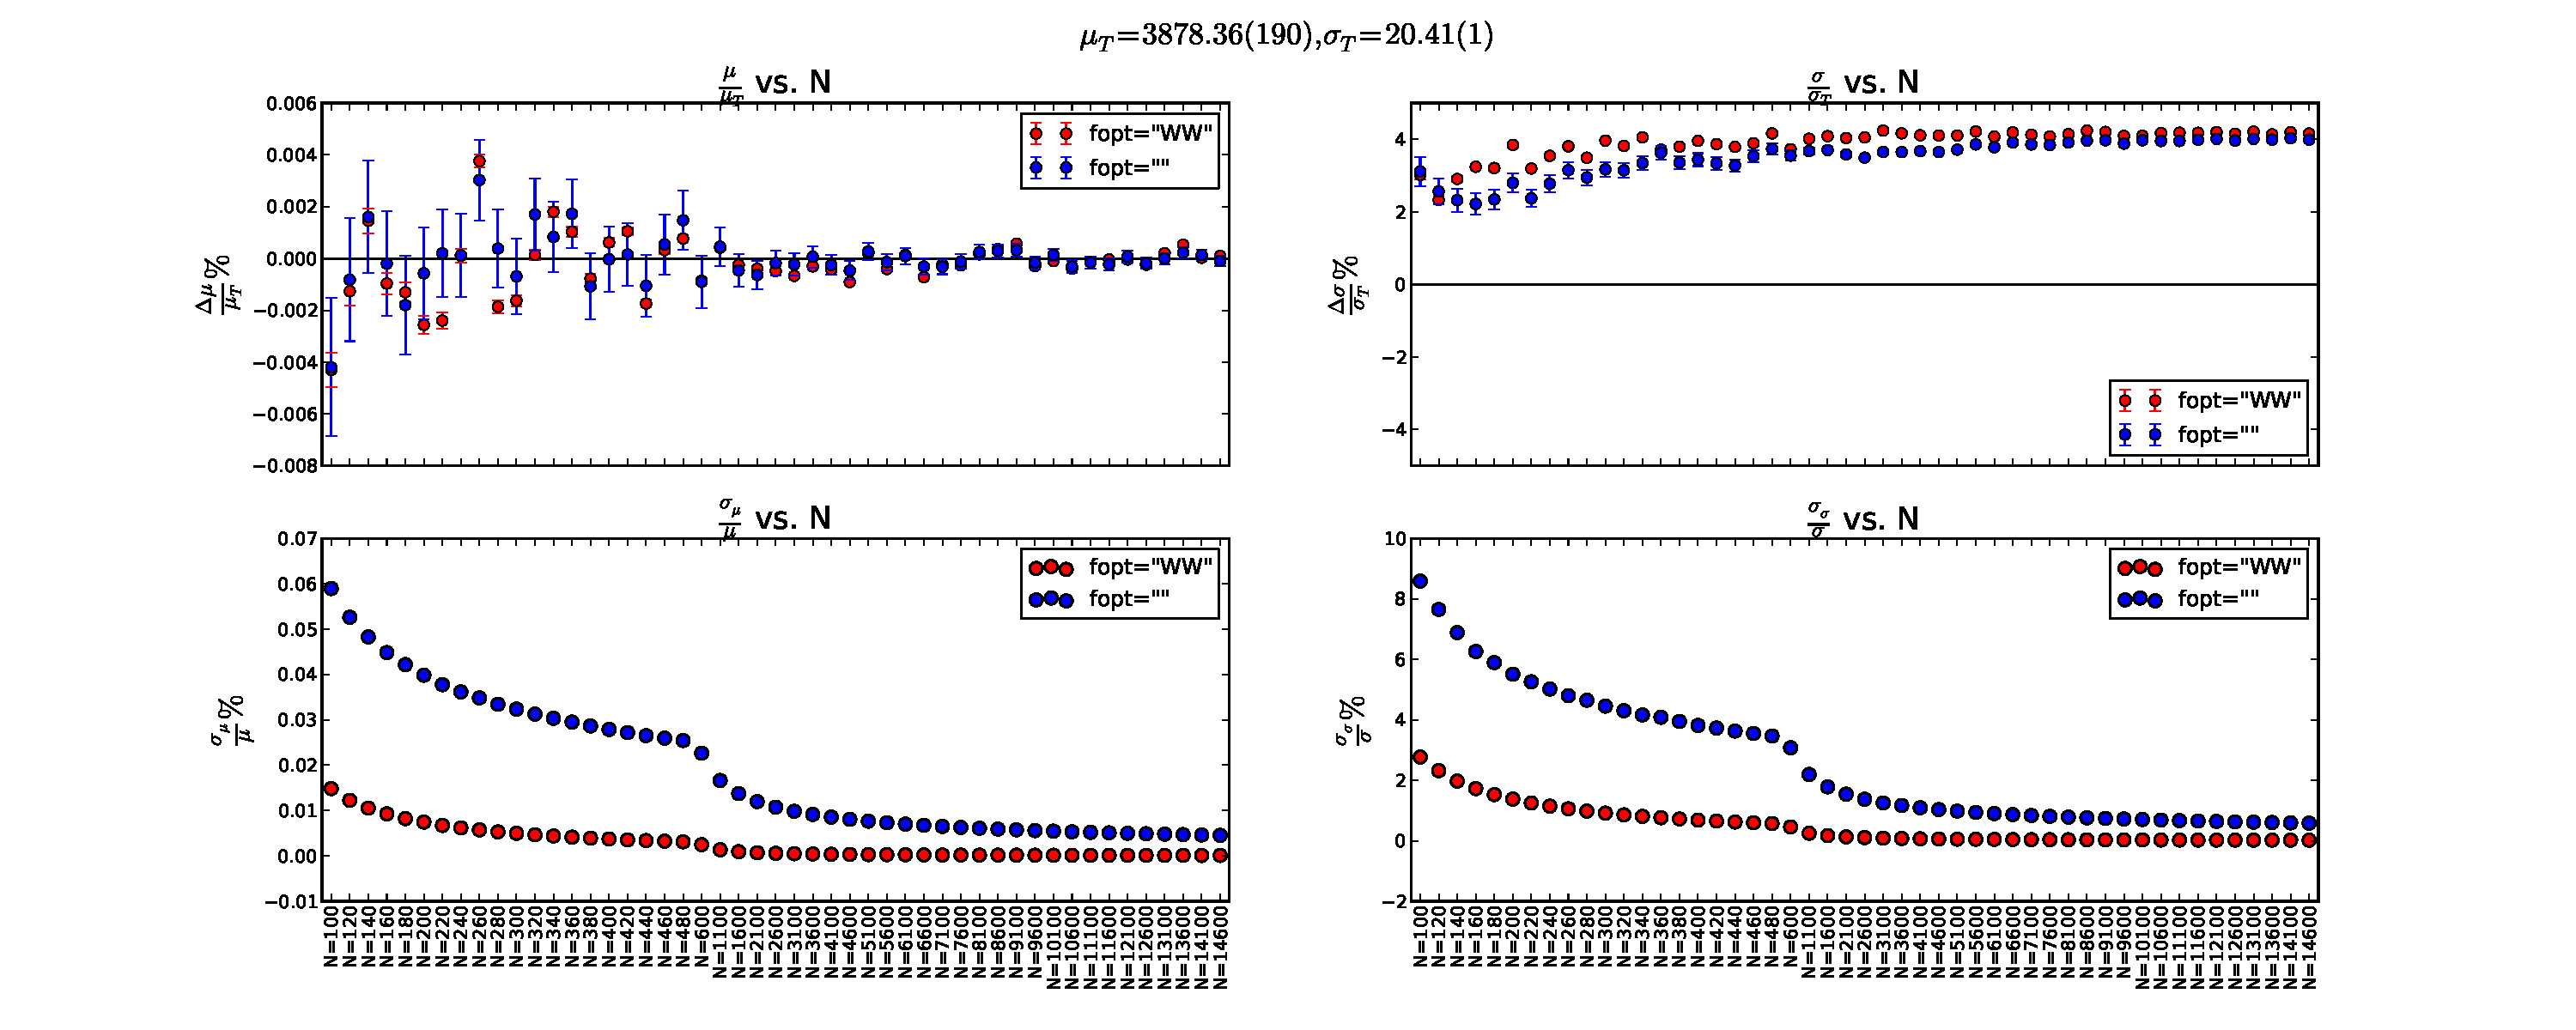
\includegraphics[height=2.5in,width=5.5in]{fit-comp_MU-190_SG-1_fit-opt-WW_binw-1.pdf}
	%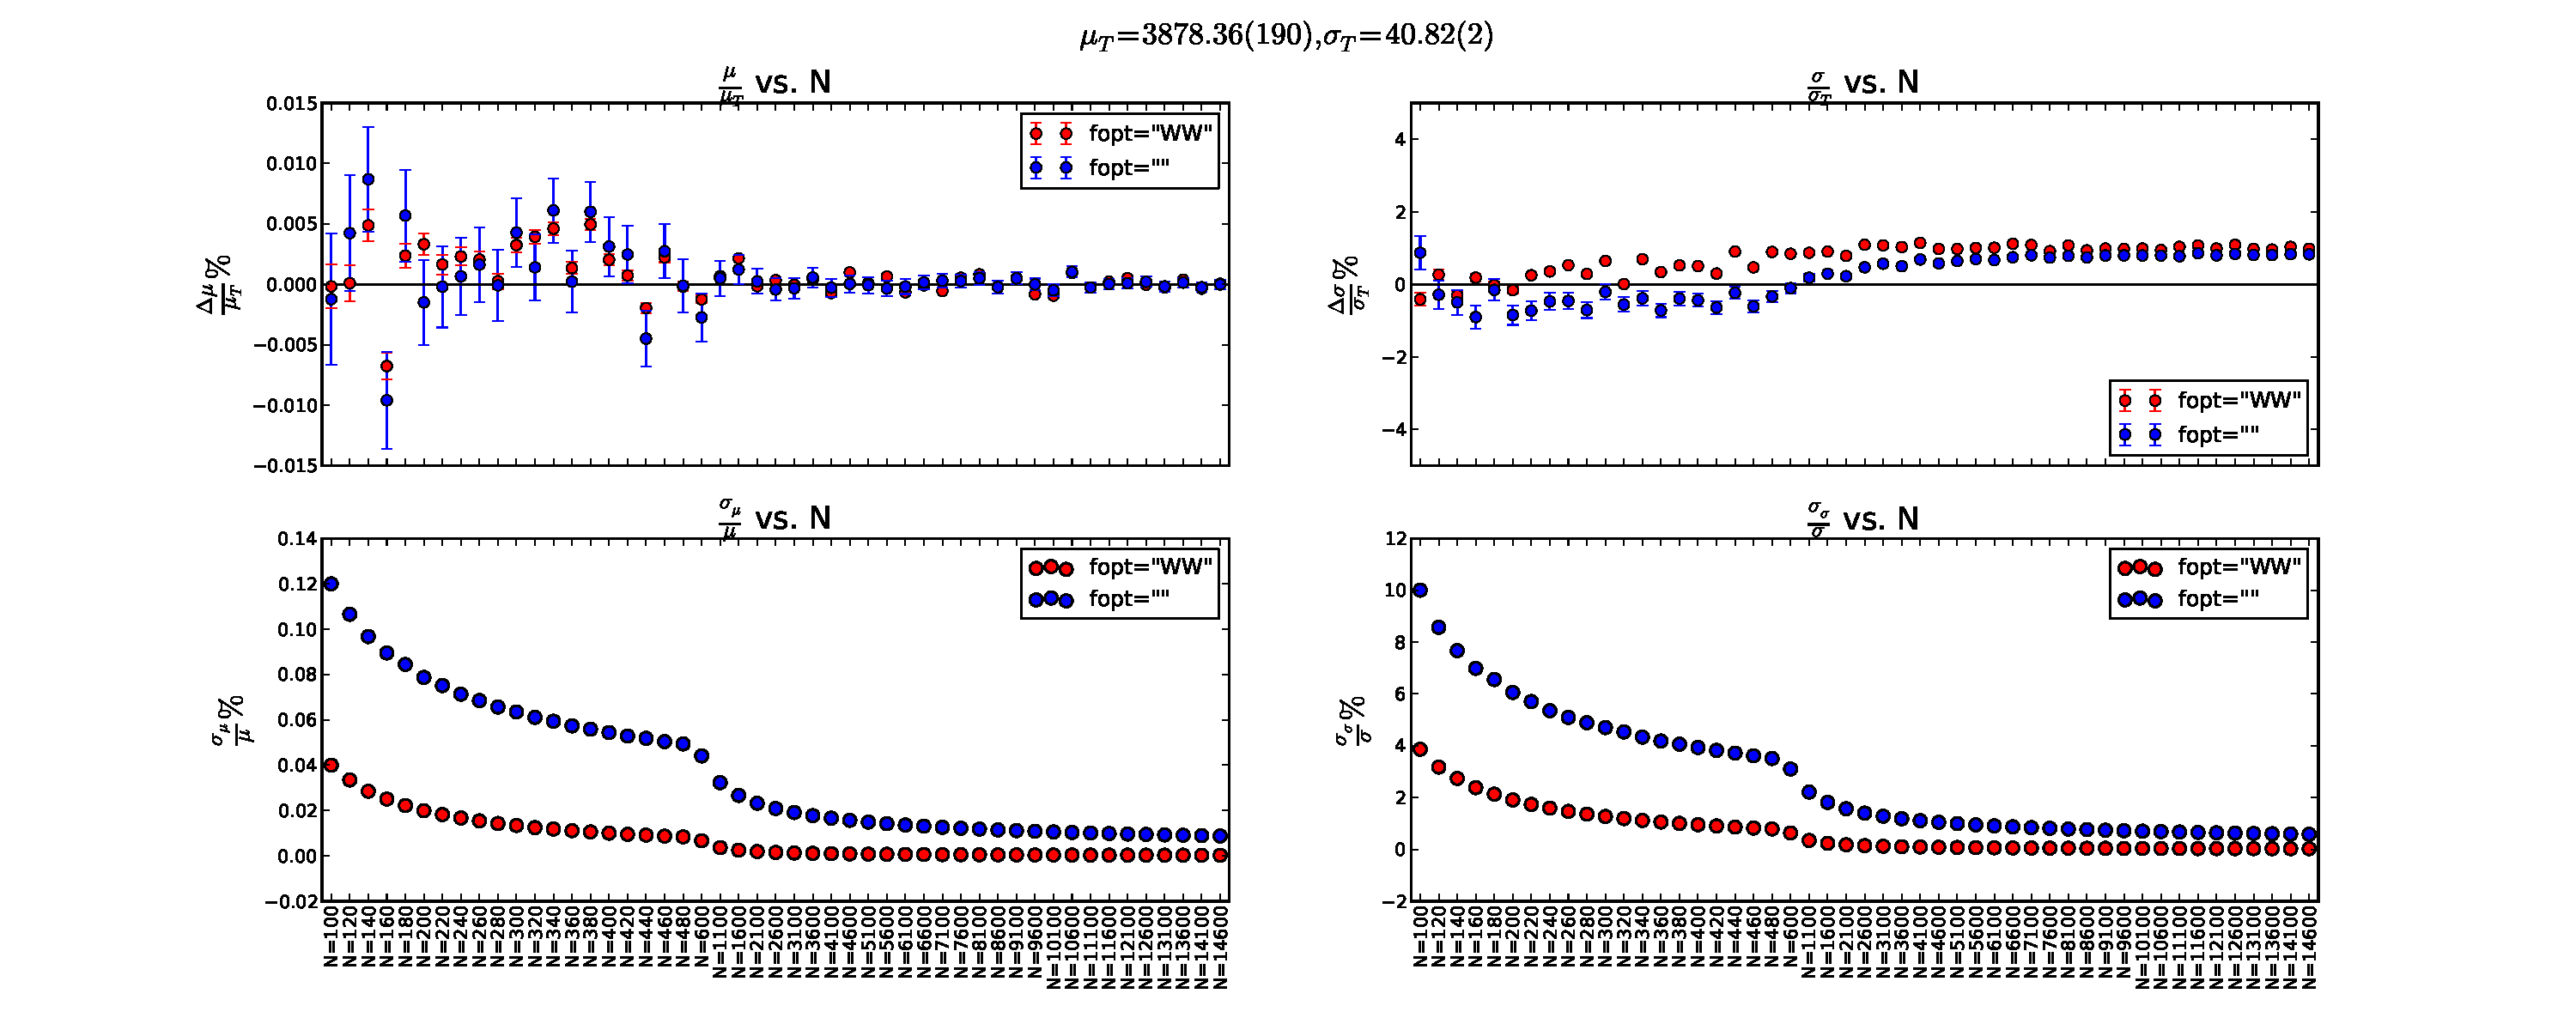
\includegraphics[height=2.5in,width=5.5in]{fit-comp_MU-190_SG-2_fit-opt-WW_binw-1.pdf}
	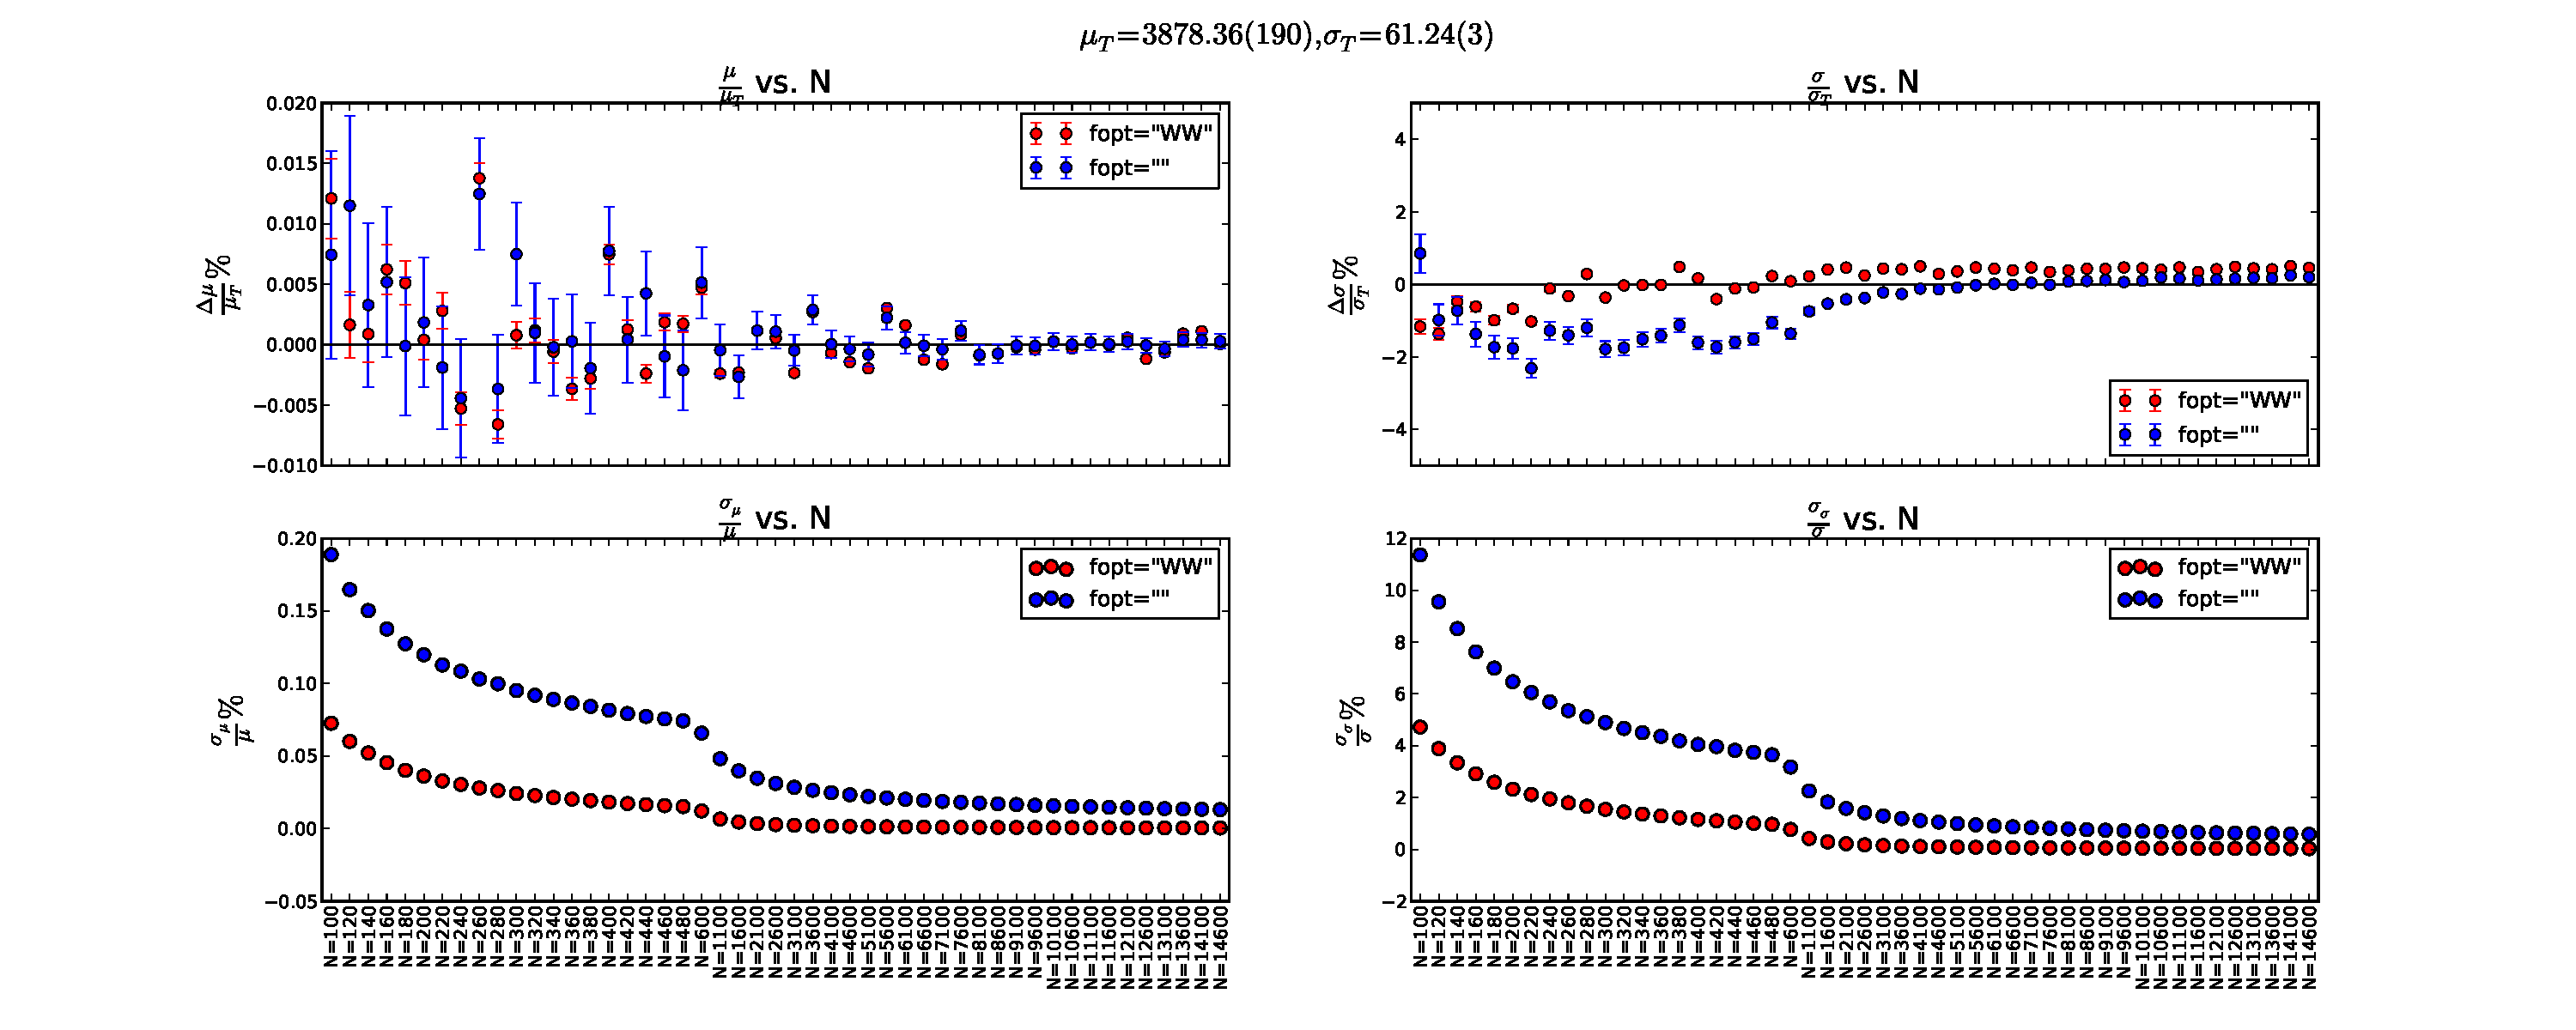
\includegraphics[height=2.5in,width=5.5in]{fit-comp_MU-190_SG-3_fit-opt-WW_binw-1.pdf}
	%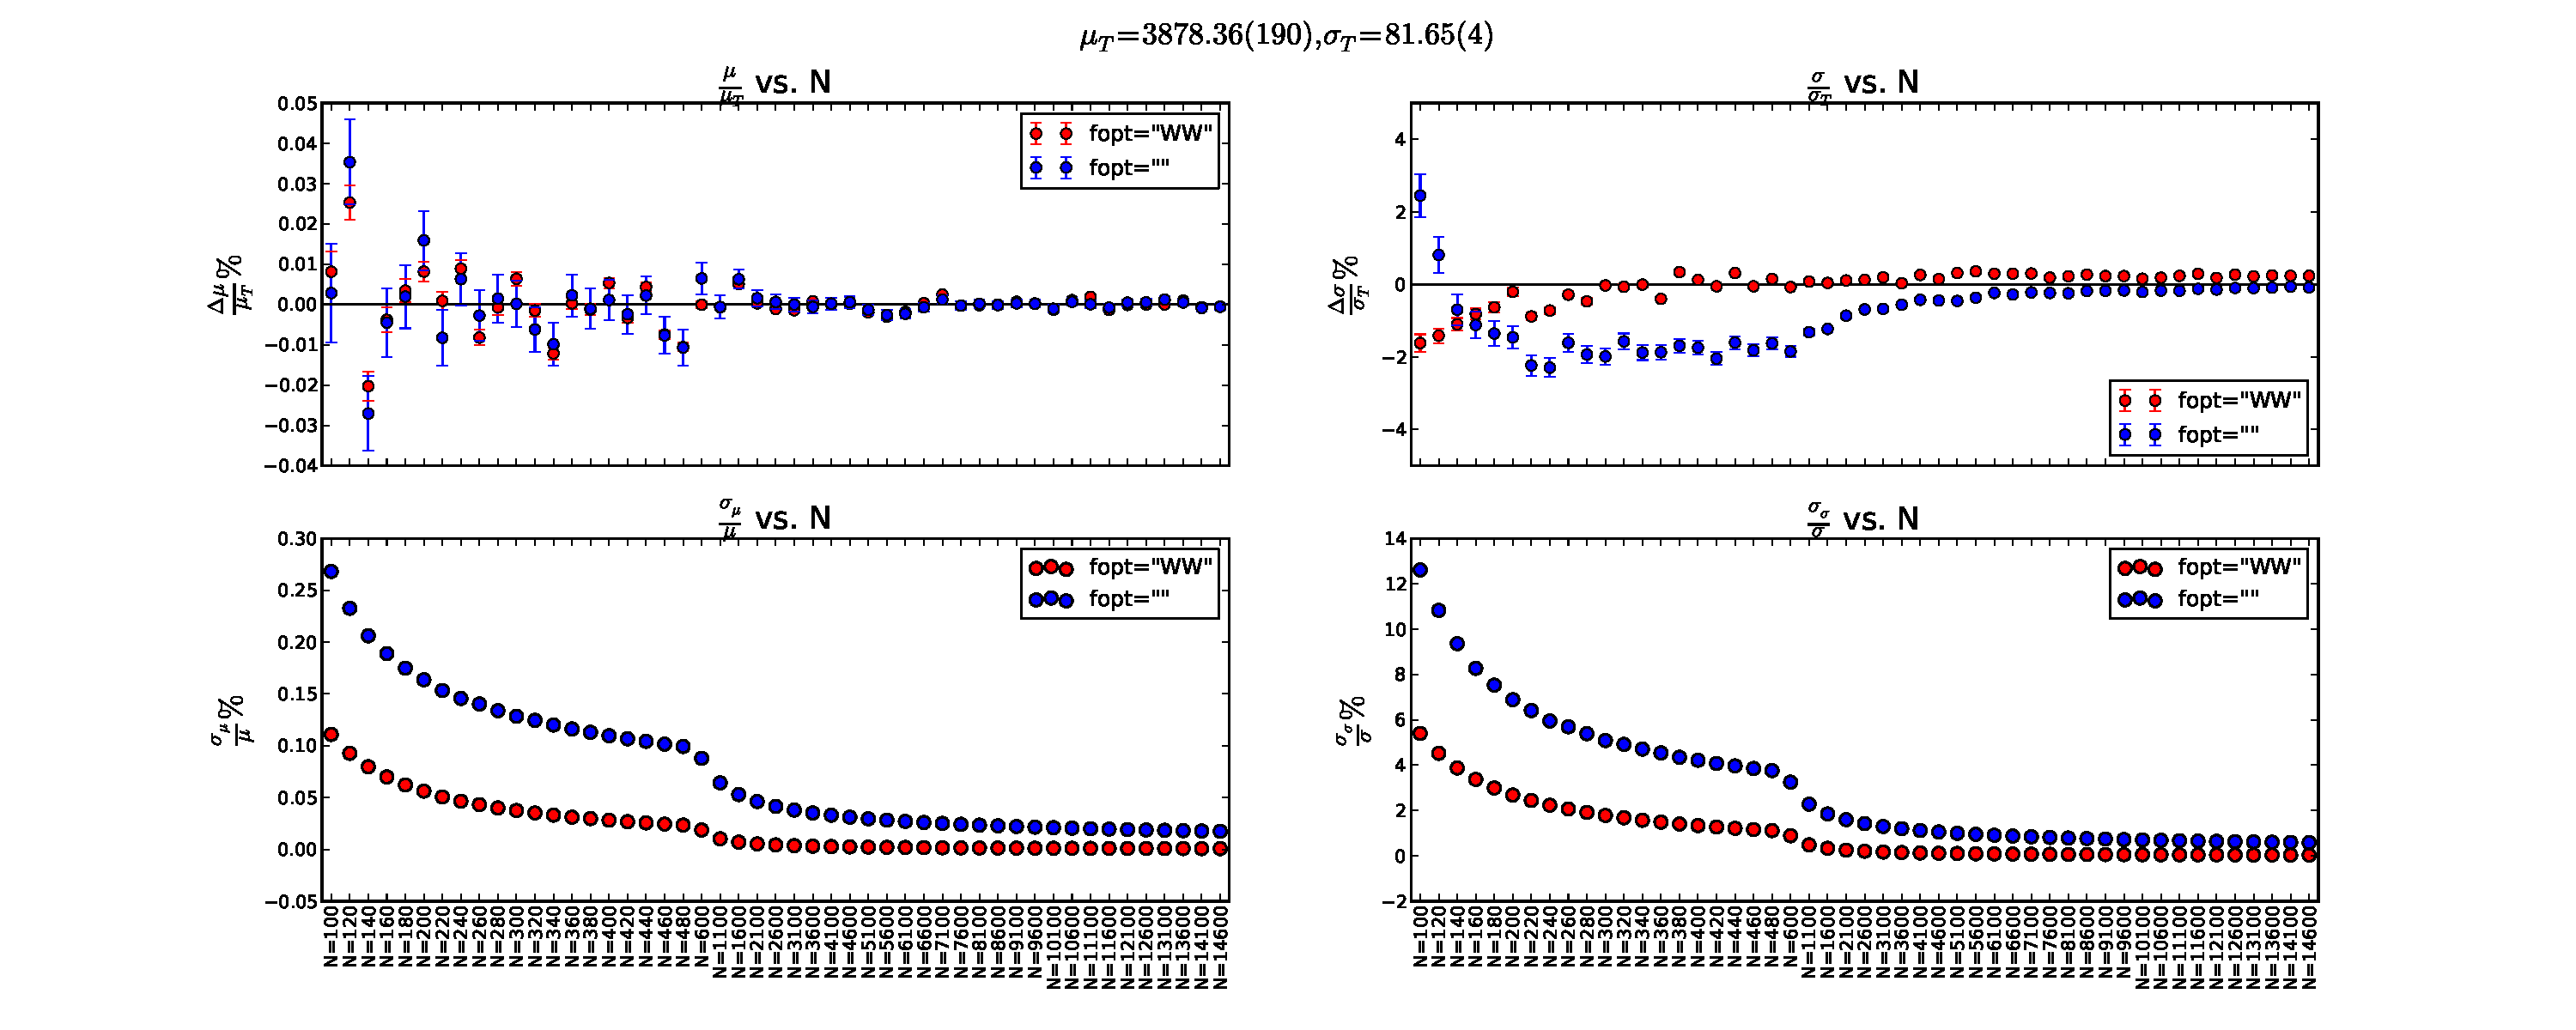
\includegraphics[height=2.5in,width=5.5in]{fit-comp_MU-190_SG-4_fit-opt-WW_binw-1.pdf}
	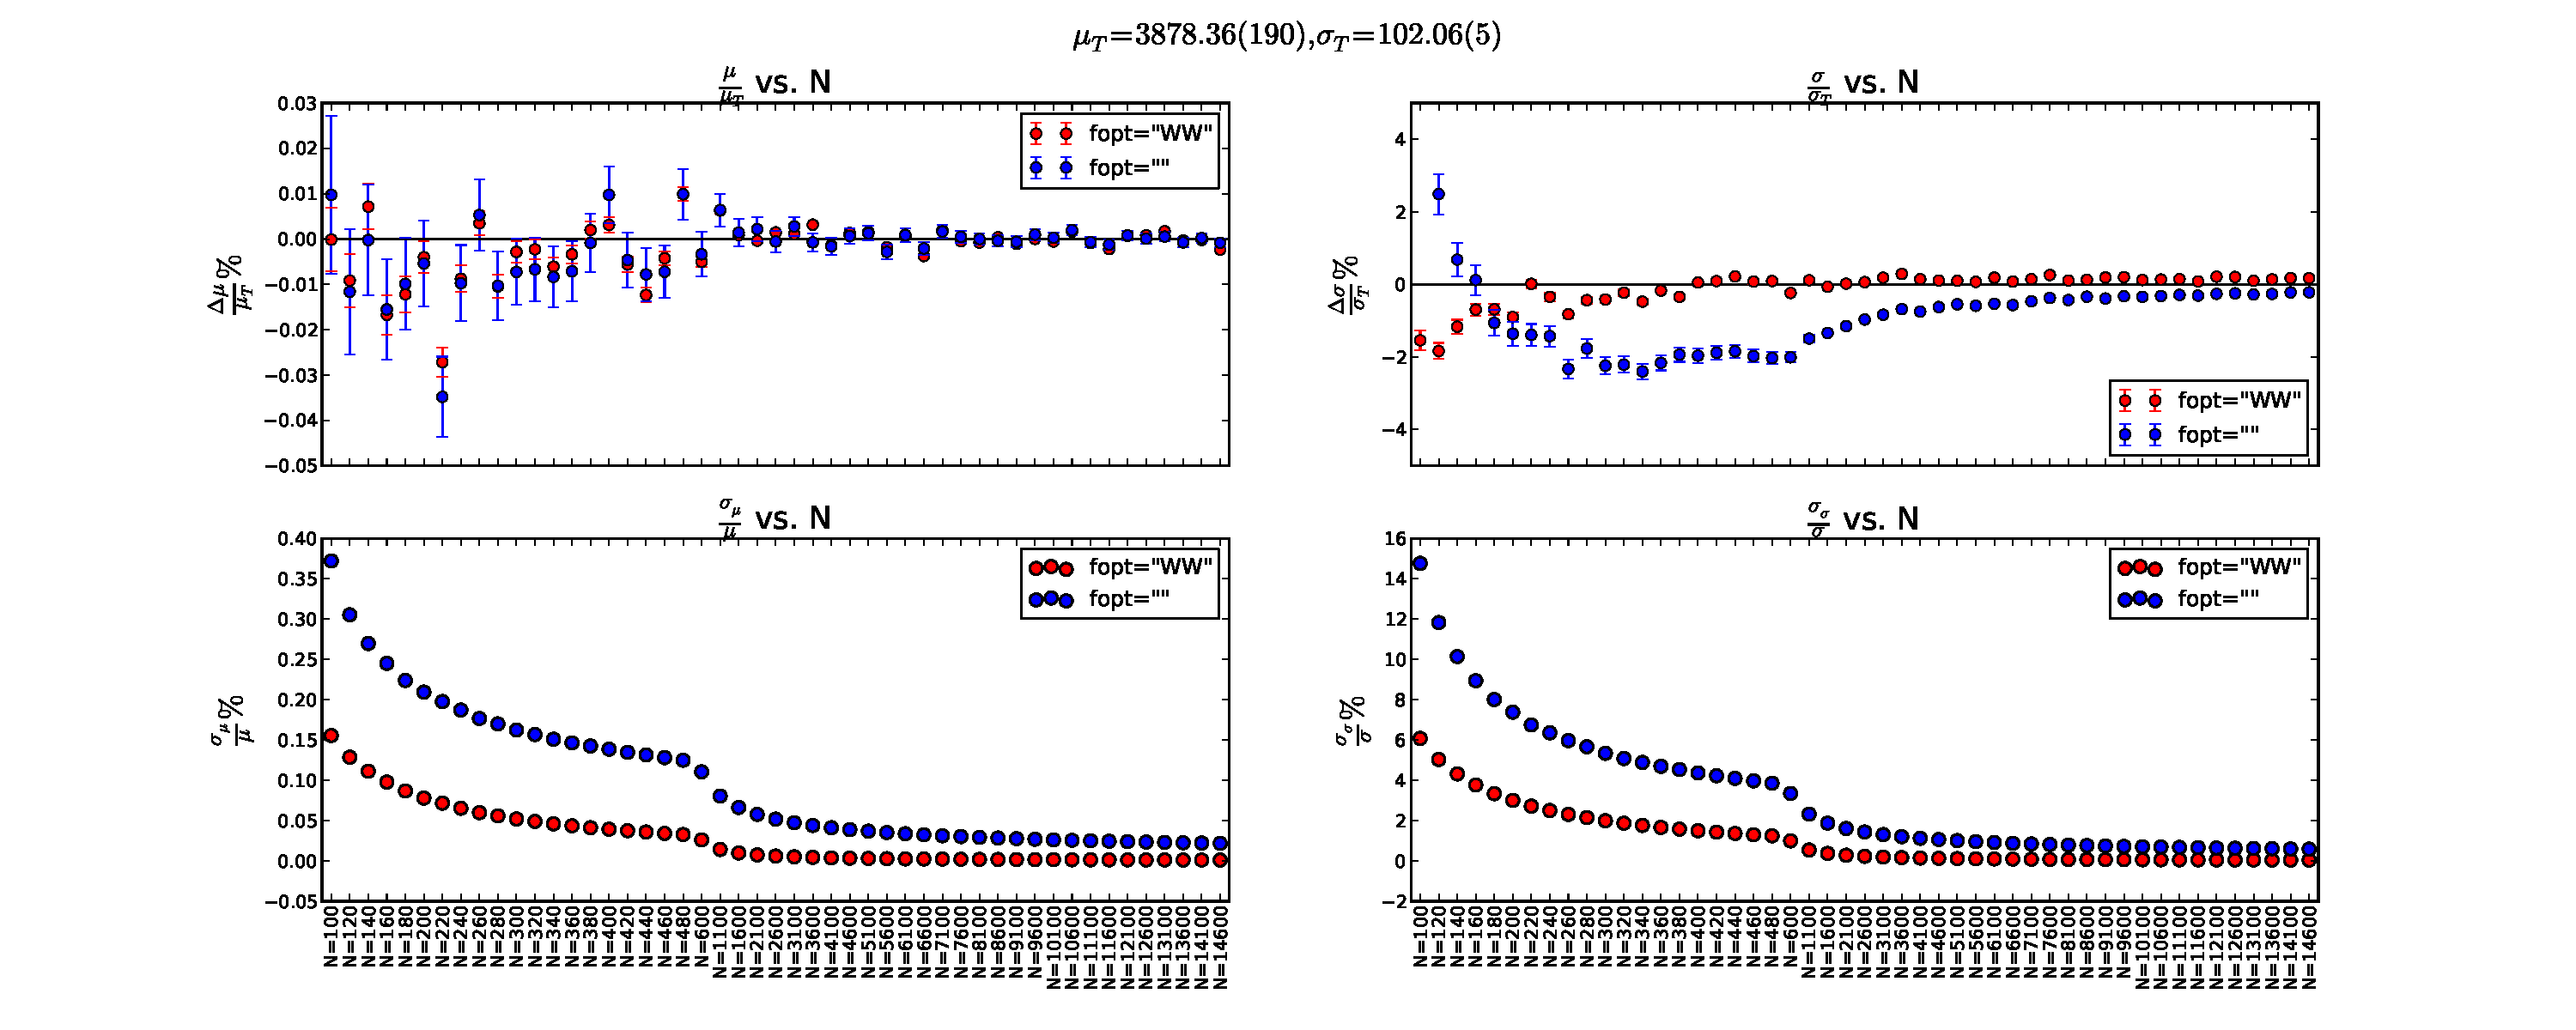
\includegraphics[height=2.5in,width=5.5in]{fit-comp_MU-190_SG-5_fit-opt-WW_binw-1.pdf}
	\caption{Extracted parameters (CSQWW and CSQ)as a function of N and $\sigma_{T}$}
	\label{fig3}
\end{figure*}

\clearpage

Following is a summary of the different ROOT Fit methods compared and their performance in the low statistical limit:

\begin{itemize}
	\item CSQ: Unstable and inaccurate in the low N region. 
	\item MLE: Significantly better than CSQ, however, is susceptible to ``outliers''.
	\item CSQ-WW: In agreement with MLE, with the following pros and cons
		\begin{itemize}
			\item [\textbf{Pros}]
			\item Not susceptible to ``outliers''.
		\end{itemize}
		\begin{itemize}
			\item [\textbf{Cons}]
			\item Error on $\sigma_{T}$ is lower than MLE.
			\item In the very low N region, can underestimate $\sigma_{T}$ by $\approx$ 2\% (\textit{May be I have conservatively simulated too low an N value and I should make it more realistic -- N$>$150 as per Fig. 1 -- and then this statement will no longer be needed})
		\end{itemize}
\end{itemize}

Therefore, given the low statistics and the need to efficiently optimize the automation program during the production of a large scale system, it was best to use the CSQ-WW method, even though the statistical errors on the estimated $\sigma_{T}$ appear to be underestimated in comparison with MLE.

This underestimation of the statistical errors by the finally used CSQ-WW method on the extracted time resolution, however, does not have a significant impact on the error on the time resolution obtained. This is because the final result is obtained by averaging the measured resolution over several points along the length of the bar and in the process the statistical error on the length averaged time resolution becomes ``insignificant'' (\textit{``insignificant'' may have to be justified in terms of non-statistical sources of error})

The only impact of using the underestimated errors of CSQ-WW is in the interpretation of the time resolution versus point-along-the-bar plot, where the underestimated errors may lead to the interpretation that the fluctuation of the data points is beyond what can be explained statistically. 

Figure 4. shows a plot for the resolution obtained for bar combination ``2-4-6'' versus the various analysis points along the length of the bar using CSQ,CSQ-WW and MLE (\textit{To bo done.}). Here it can be seen that the results from CSQ-WW underestimate the errors relative to CSQ and MLE. Additionally, here it can be directly observed that the CSQ method tends to underestimate the time resolution and MLE, due to ``outliers'', overestimates the time resolution and causes the resolution versus position data to no longer agree with a parabola fit.  

\begin{figure*}[ht]
	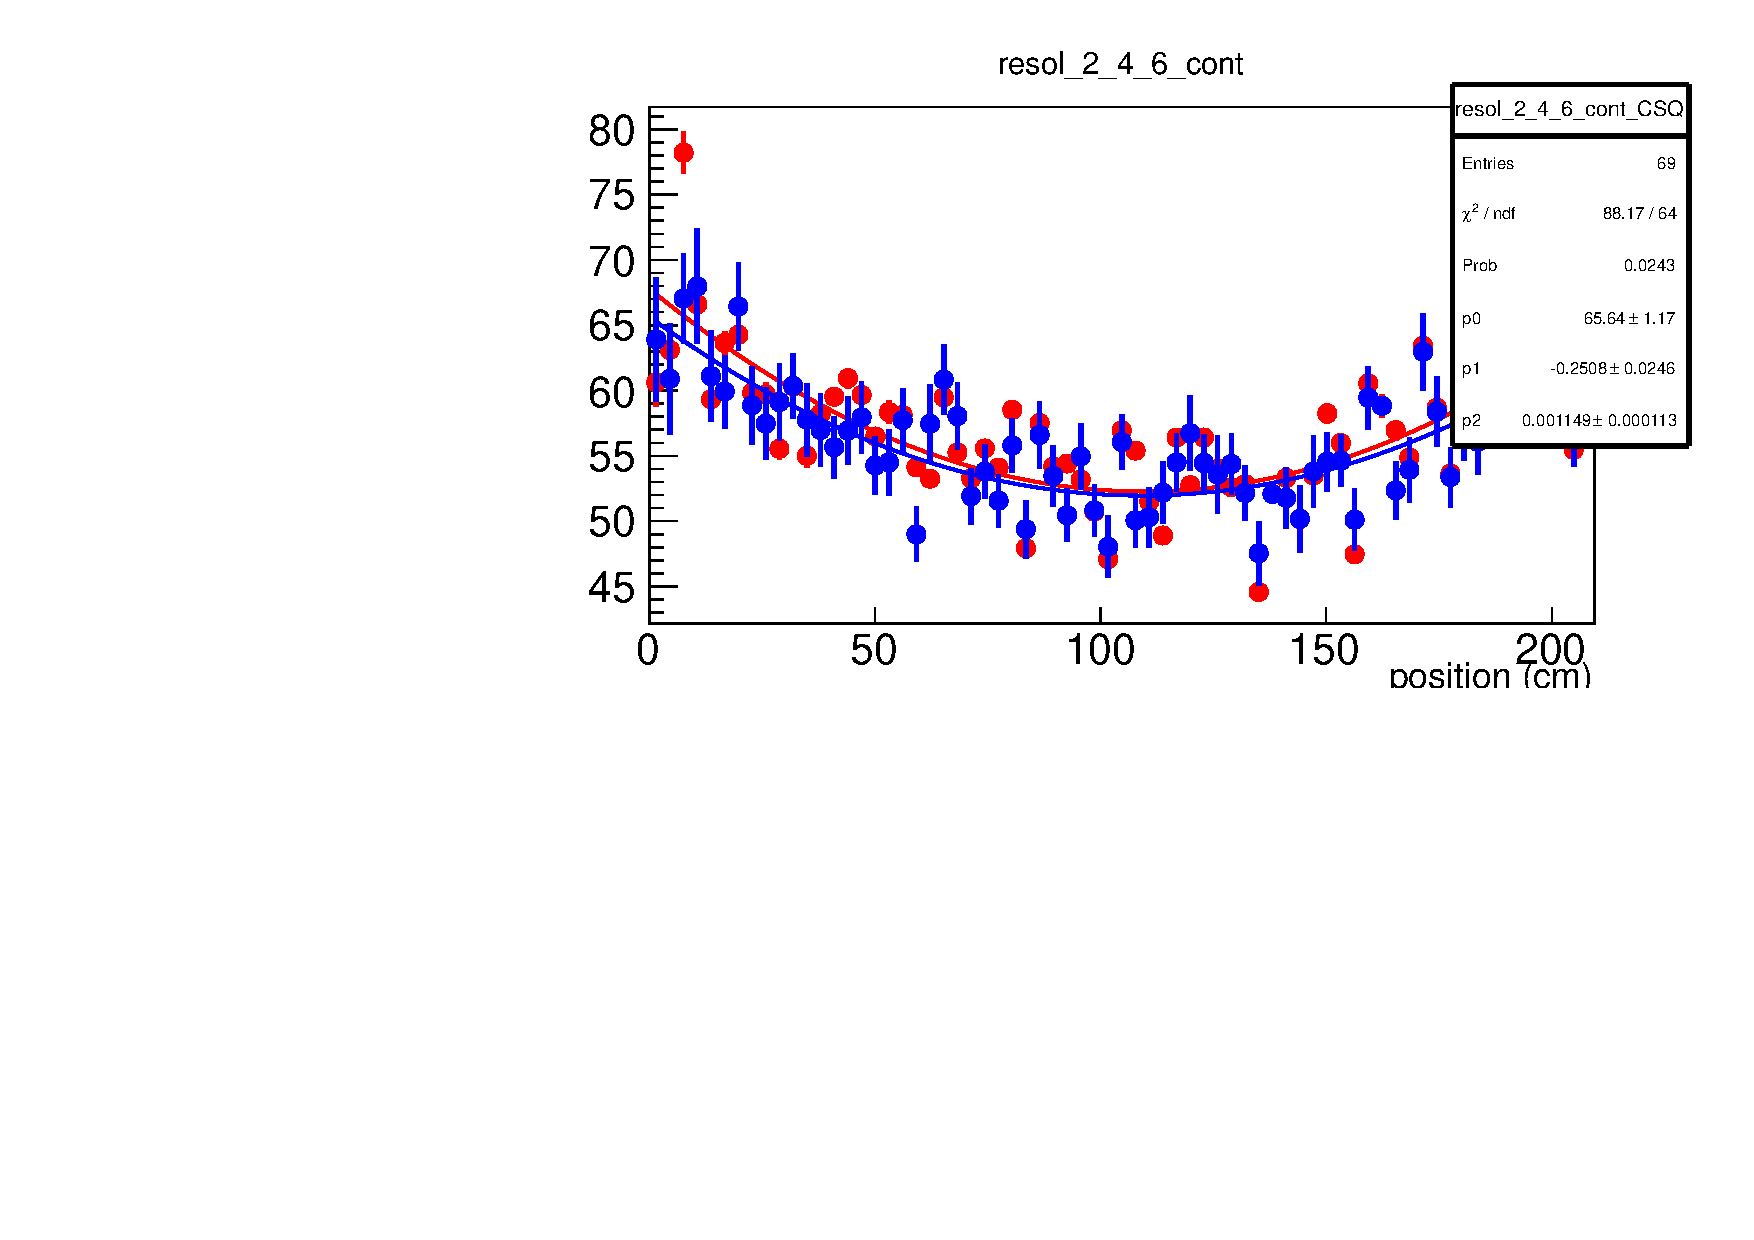
\includegraphics[height=2.5in,width=5.5in]{res_vs_pstn.pdf}
	\caption{Demo underestimation of errors by CSQWW by comparing with CSQ by way of resolution vs. point plot (I had previously compared with CSQ, but with binw=0.25, CSQ is no longer valid to compare with if sets with binw=0.25 is to be used) }
	\label{fig4}
\end{figure*}  

\clearpage


\end{document}